\documentclass[serif,mathserif]{beamer}
\usepackage{amsmath, amsfonts, epsfig, xspace}
\usepackage{algorithm,algorithmic}
\usepackage{pstricks,pst-node}
\usepackage{multimedia}
\usepackage[normal,tight,center]{subfigure}
\setlength{\subfigcapskip}{-.5em}
\usepackage{beamerthemesplit}
\usetheme{lankton-keynote}

\author[Tejaswi KC, Raj Krishnan]{Group 11 \\ Tejaswi KC \quad Raj Krishnan \\ 140010020 \quad 140010007}

\title[PyAlpha\hspace{2em}\insertframenumber/\inserttotalframenumber]{PyAlpha: Final Report}

\date{November 21, 2016}

\institute{Indian Institute of Technology, Bombay}

\begin{document}

    \maketitle

    \begin{frame}

        \frametitle{Tasks}

        \begin{itemize}
            \item Build a python module to handle the purchase and sale of stocks
                  as per current prices on the share markets
            \item Build a module to compute the quality of various alphas
                  (weights for various stocks)
            \item Hosted at \url{https://github.com/raj-krishnan/PyAlpha}
        \end{itemize}

    \end{frame}

    \begin{frame}

        \frametitle{Tests}

        \textbf{Testsuite:}
        \begin{figure}
            \centering
            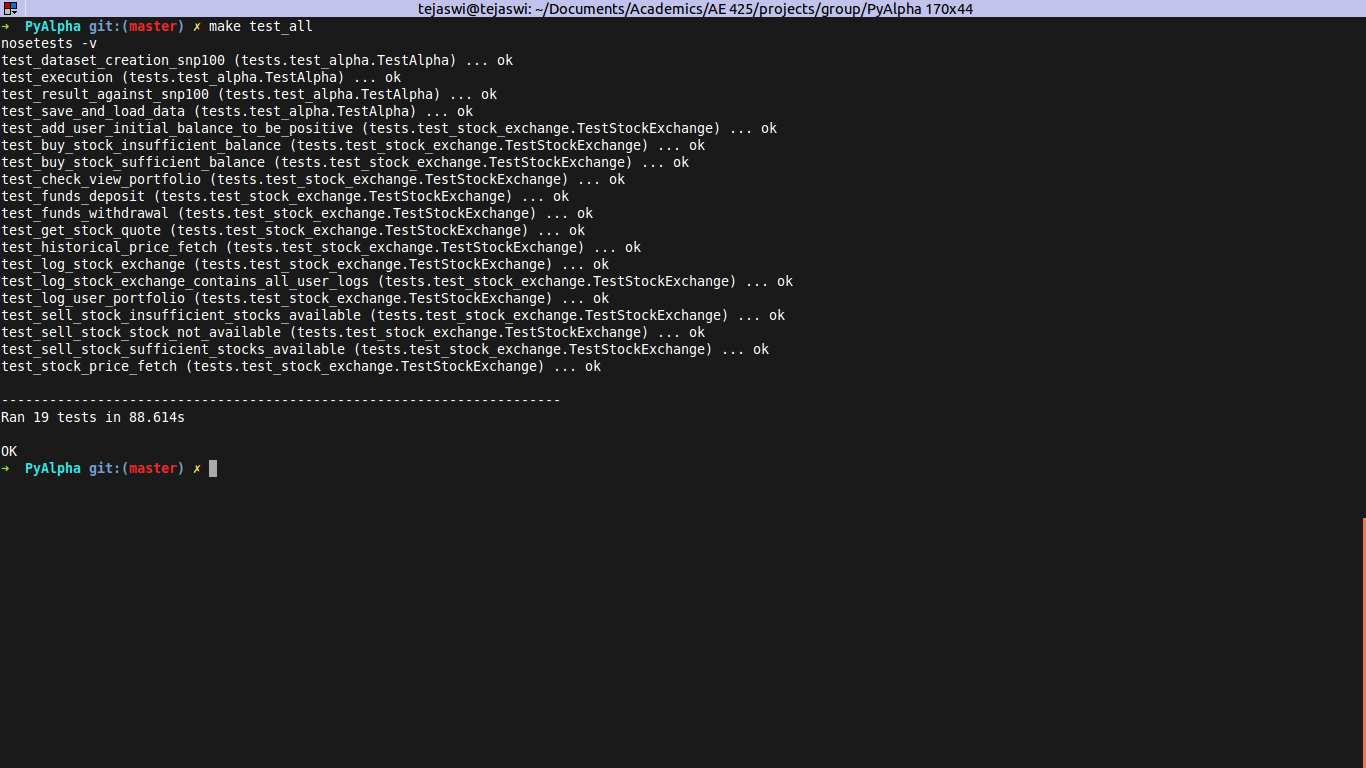
\includegraphics[width = \linewidth]{testsuite.png}
        \end{figure}

    \end{frame}

    \begin{frame}{Coverage}

        \textbf{Coverage: 92\%}
        \begin{figure}
            \centering
            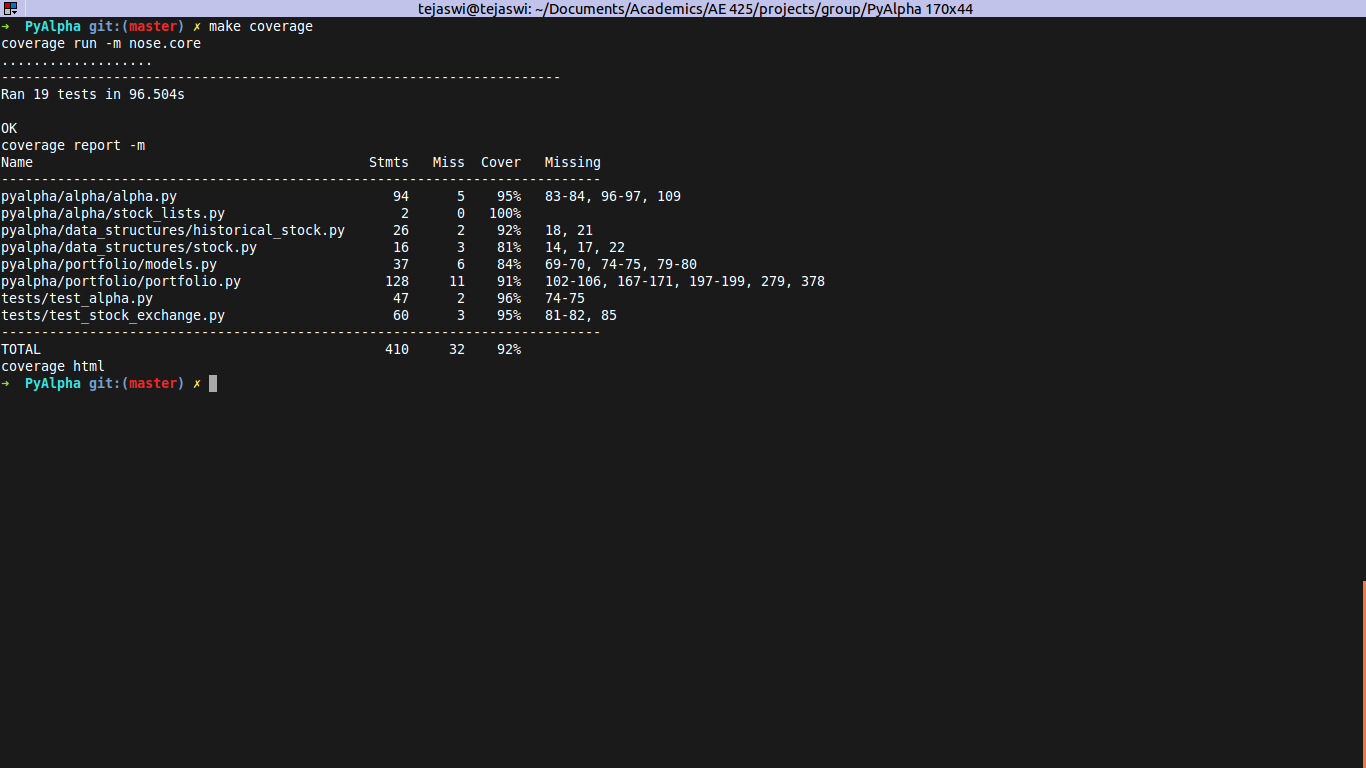
\includegraphics[width = \linewidth]{coverage.png}
        \end{figure}

    \end{frame}

    \begin{frame}{Automation}

        \begin{itemize}
            \item A root level makefile is available
            \item setup.py is available
            \item Continuous Integration using \href{https://travis-ci.org/raj-krishnan/PyAlpha}{Travis}
            \item Coverage Testing using \href{https://coveralls.io/github/raj-krishnan/PyAlpha}{Coveralls}
        \end{itemize}

    \end{frame}

    \begin{frame}{Git commit graphs}

        \begin{figure}[h]
            \centering
            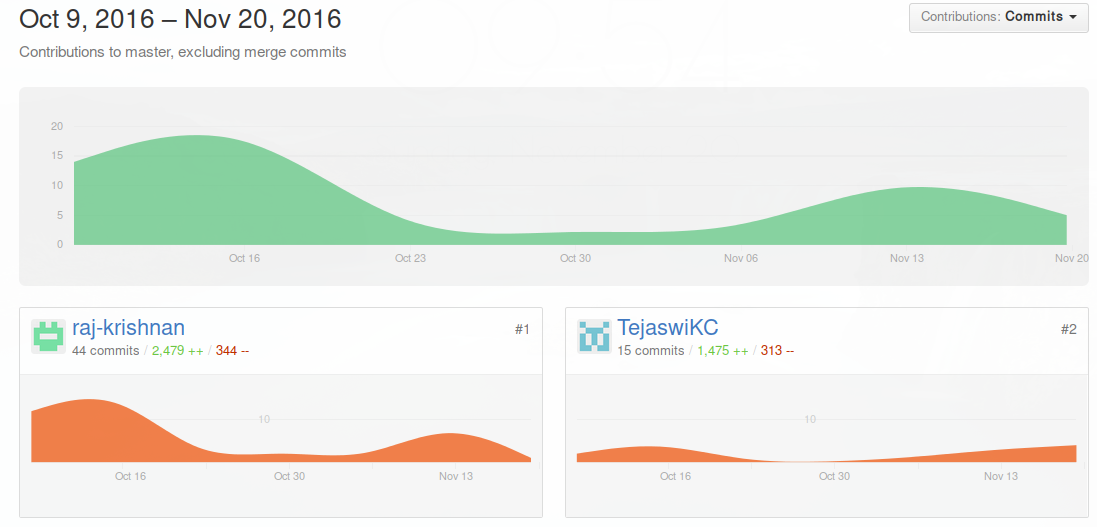
\includegraphics[width=\linewidth]{commits.png}
        \end{figure}

    \end{frame}



    \begin{frame}{Documentation}

        \begin{itemize}
            \item Documentation hosted at \url{http://pyalpha.readthedocs.io/}
            \item Installation Instructions, tutorials and docstrings available
        \end{itemize}

        \begin{figure}
            \centering
            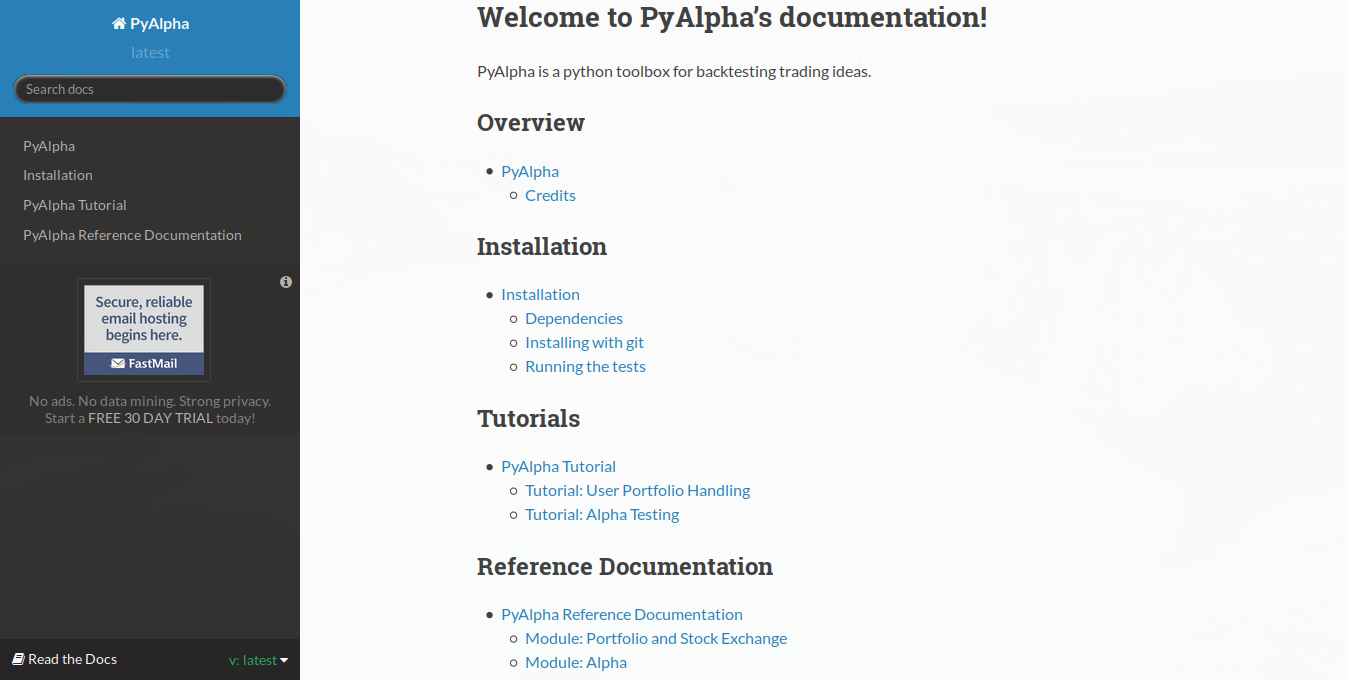
\includegraphics[width = \linewidth]{docs.png}
        \end{figure}


    \end{frame}

    \begin{frame}{Code cleanliness and Usage}

        \begin{itemize}
            \item Following PEP8
            \item Usage of Stock Exchange:
            \begin{itemize}
                \item Create an instance of StockExchange
                \item Add users to the stock exchange
                \item Each user can individually buy and sell stocks
                \item Logs for individual users and entire stock exchange available
            \end{itemize}
            \item Usage of Alpha Testing Module
            \begin{itemize}
                \item Inherit the Alpha abstract class and define the method alpha
                \item Set time period and stocks to be taken under consideration
                \item Create dataset and run simulation
                \item Daily returns and turnover are now available
            \end{itemize}
            \item Tutorials are available at \url{http://pyalpha.readthedocs.io/en/latest/tutorials/tutorial.html}
        \end{itemize}

    \end{frame}

    \begin{frame}

        \frametitle{Portfolio Handling Demo}

        \begin{figure}[h]
            \centering
            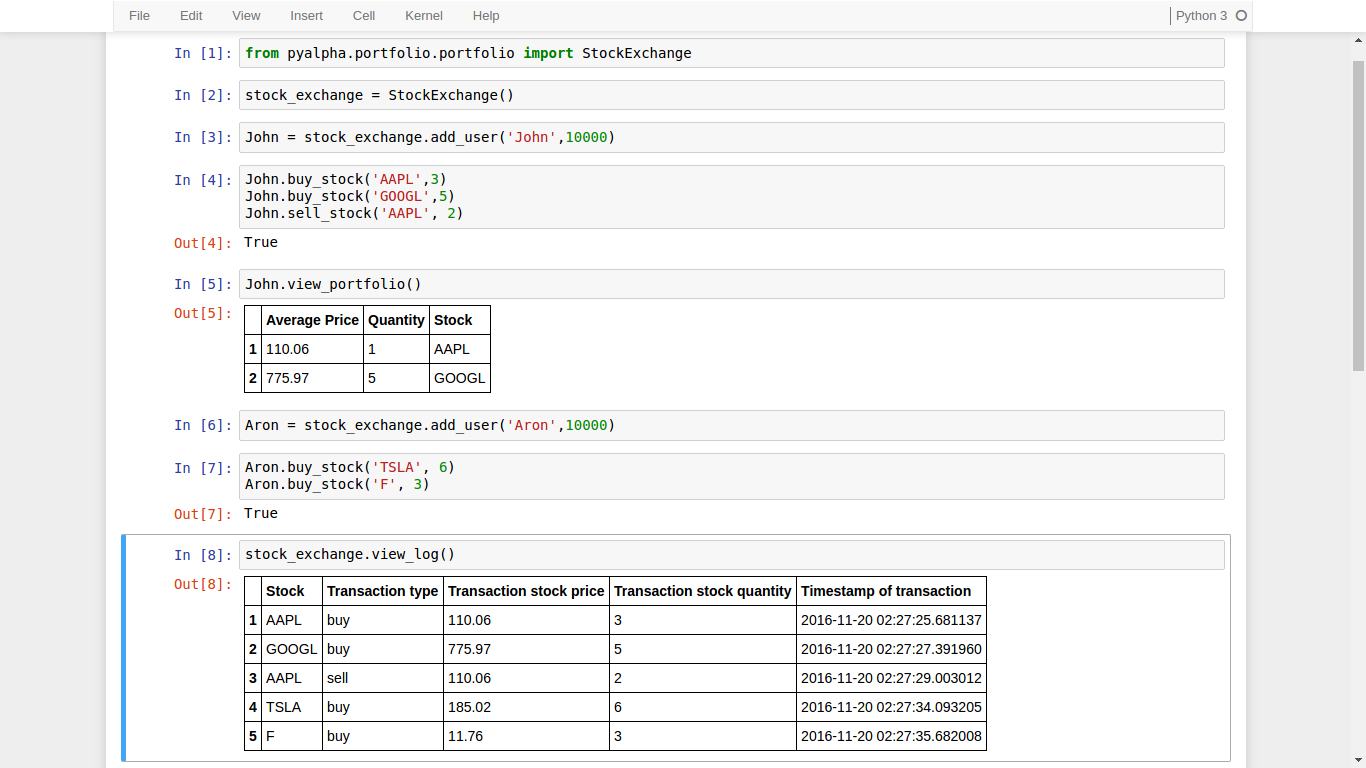
\includegraphics[width=\linewidth]{portfolio.png}
        \end{figure}

    \end{frame}

    \begin{frame}

        \frametitle{Alpha Testing Demo}

        \begin{figure}[h]
            \centering
            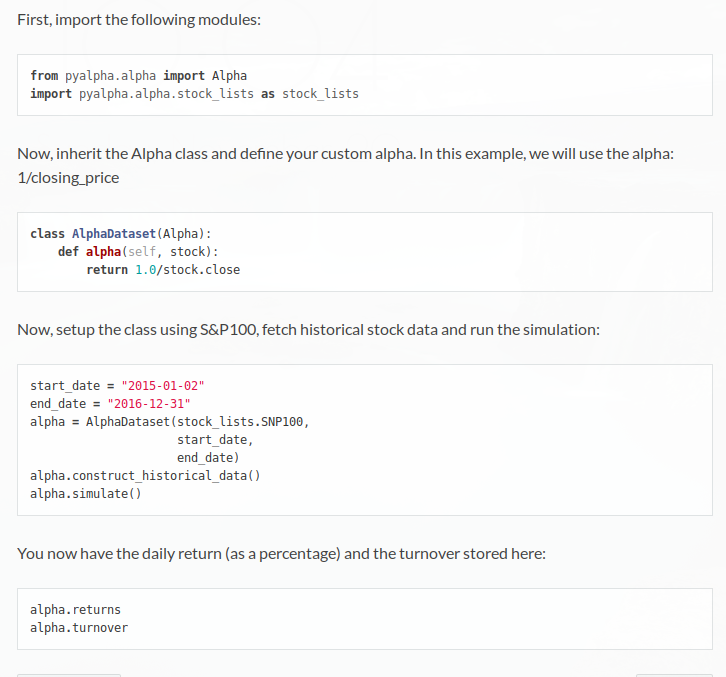
\includegraphics[height=7.5cm]{alpha_tutorial.png}
        \end{figure}

    \end{frame}

    \begin{frame}

        \frametitle{Dependencies}

        \begin{itemize}
            \item Numpy
            \item pandas
            \item peewee: For handling databases
            \item ystockquote: For fetching data from Yahoo Finance
        \end{itemize}

    \end{frame}

    \begin{frame}
        \frametitle{Issues Faced}

        \begin{itemize}
            \item Some stocks are not available using ystockquote, due to issues with Yahoo Finance
            \item Examples include: Paypal (PYPL), Fortive Corp (FTV) etc
            \item Issue has already been raised: \url{https://github.com/cgoldberg/ystockquote/issues/43}
        \end{itemize}
    \end{frame}

    \begin{frame}
        \centering \huge{Thank You!}
    \end{frame}

\end{document}
